\section{Procedure}\label{Sect:procedure}
\subsection{Quantum Mechanical Data}\label{Sect:procedureData}
%\subsection{}
%
% Talk about the data file given to me by Brother Nelson
%
%
%
%
%
%
%
\par Brother Nelson gave me a bunch of data...
\par Because effective models could be contructed with the Lennard-Jones potential, a similar model could potentially be used to train from and predict useful data faster than current models. The data discussed and used in this section was generated by and received from Lance Nelson. It was generated using a particularly complicated model that incorporated principles of math and quantum mechanics that are beyond the scope of this paper. It is important to understand that the process of obtaining said data was computationally expensive and difficult. The culmination of this research is to produce a simpler model that can be trained on the given data then reproduce expected energies within a range of reasonable error. For a reference, Figure \ref{histEnergy} shows a histogram of all the configuration energies in the data set.

\begin{figure}[h]
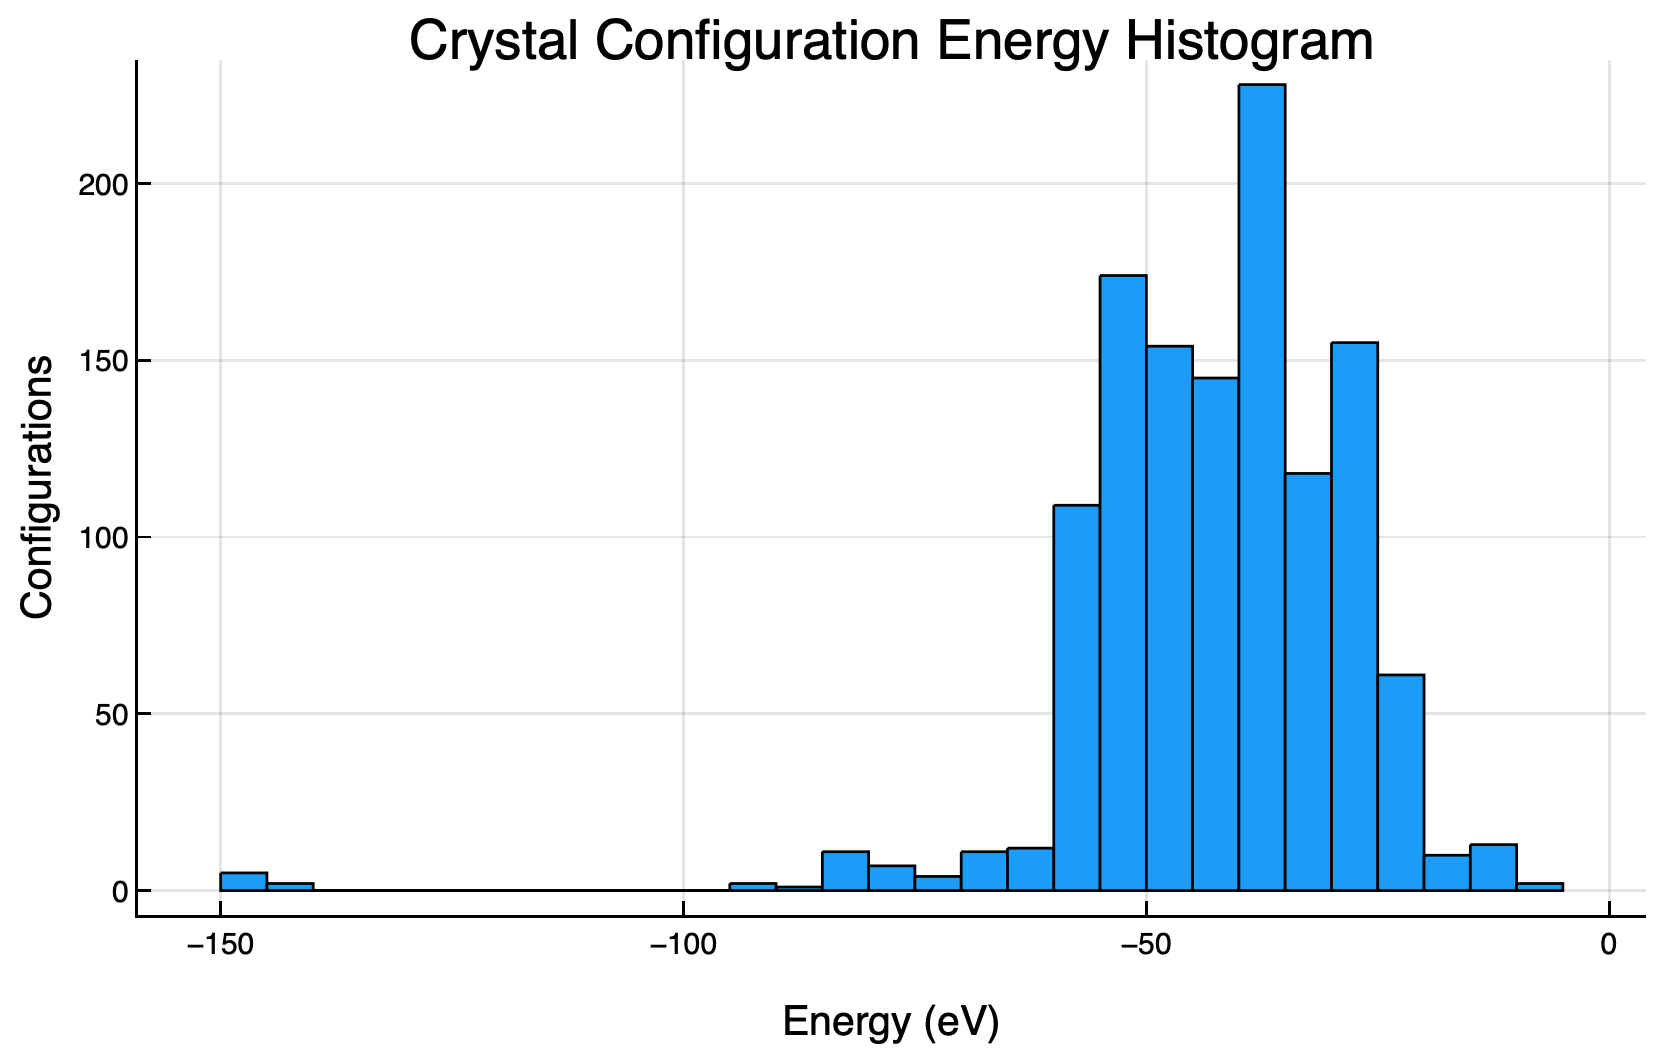
\includegraphics[scale = 0.3]{Figures/UnitCellEnergies}
\caption{A histogram showing all the configuration energies in the original data file. The majority lie within the $-20$eV to $-60$eV range, with a few outliers around $-150$eV.
\label{histEnergy}} 
\end{figure}

\par Each configuration in the data represents a unique primitive unit cell. A unit cell is the building block of any crystal structure. Each unit cell is an identical copy of another, with the same shape, size, and contents. A \textit{primitive} unit cell is the smallest possible unit cell which contains only one of each uniquely positioned atoms in the crystal. An example of a primitive unit cell configuration can be seen in Figure \ref{primitiveUnitCells}.

\begin{figure}
  \begin{subfigure}{0.25\textwidth}
    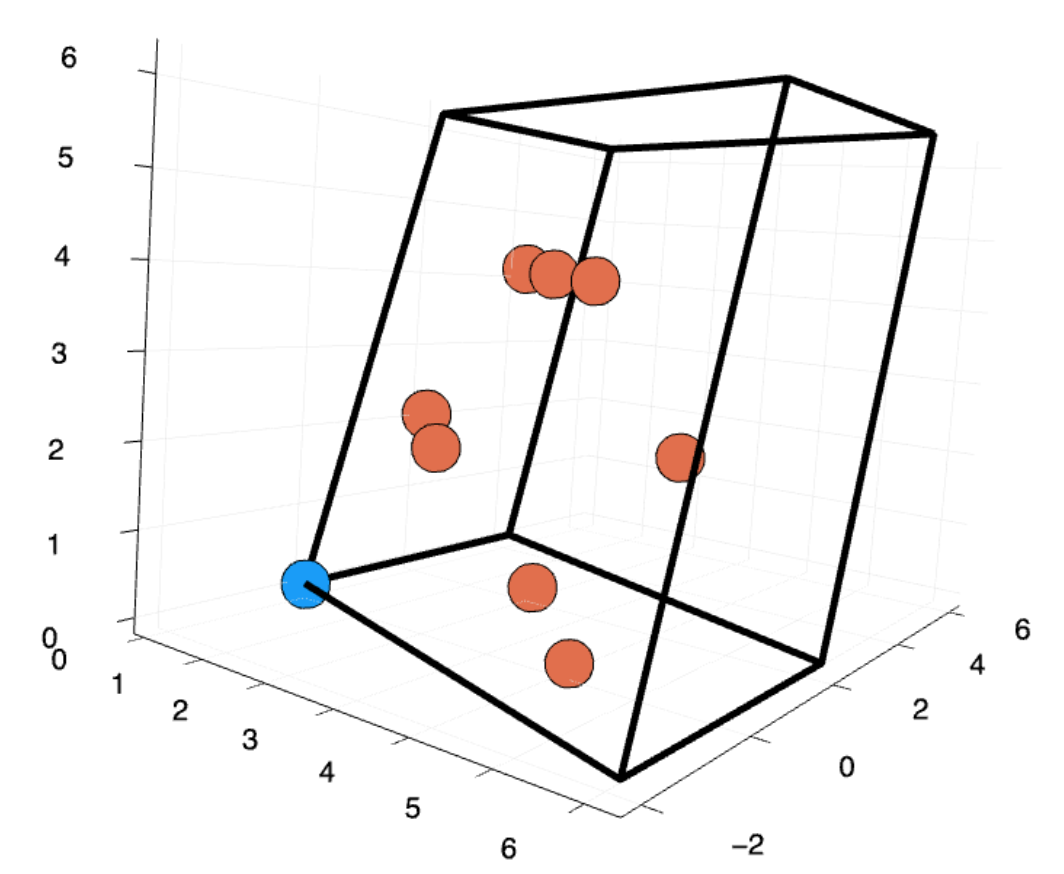
\includegraphics[width=\linewidth]{Figures/primitiveCell1}
    %\caption{First subfigure} 
    \label{primitiveFirst}
  \end{subfigure}%
  \hspace*{\fill}   % maximize separation between the subfigures
  \begin{subfigure}{0.23\textwidth}
    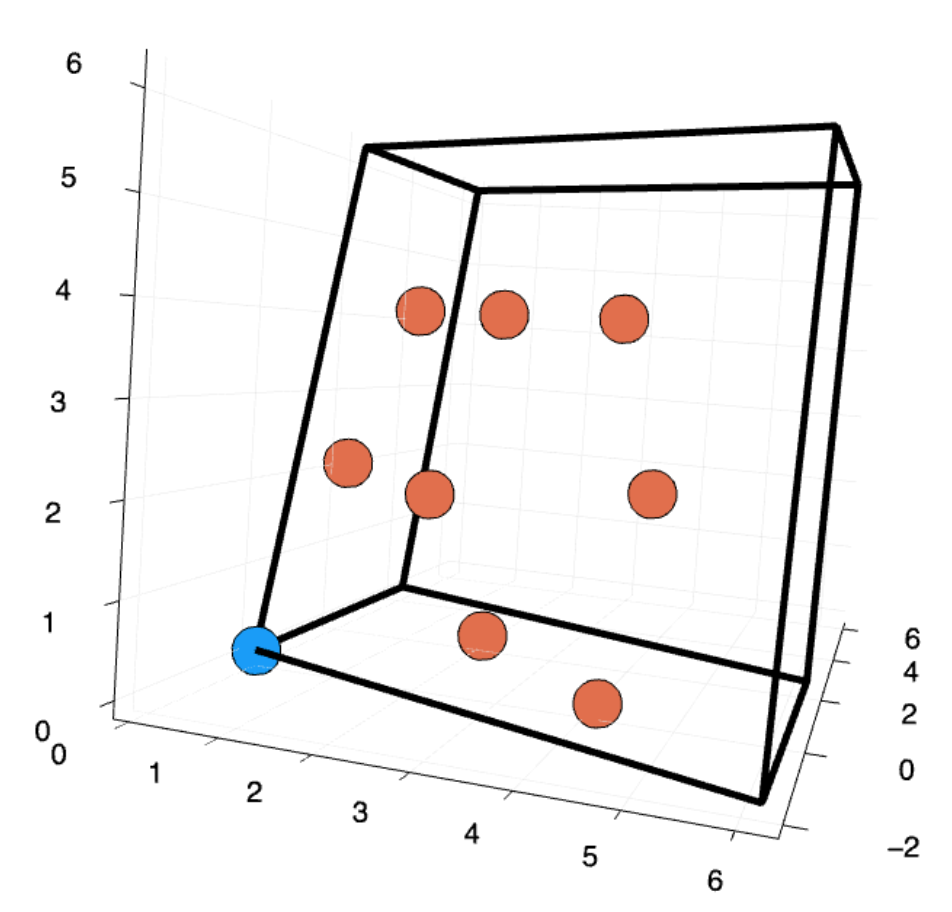
\includegraphics[width=\linewidth]{Figures/primitiveCell2}
    %\caption{Second subfigure} 
    \label{primitiveSecond}
  \end{subfigure}%
\caption{The primitive unit cell for configuration 65 from two different perspectives. The blue point is the single Ag atom while each red point shows each Pt atom in said configuration.} \label{primitiveUnitCells}
\end{figure}

\par In order to use the data in the \textit{.txt} file, it needs to be parsed into vectors that can be easily manipulated. An example of the data being parsed can be seen in Figure \ref{system2data}. The ``str" can be identified in the first line to begin each new system. The number on the second line is the lattice parameter followed by three lattice vectors in $(i,j,k)$ coordinates. The following line contains two numbers, the first is the number of silver (Ag) atoms in the unit cell and the second is the number of platinum (Pt) atoms. In direct coordinates (in terms of the lattice vectors) we are given the positions of each silver and platinum atom in order. The last line in this system tells the total potential energy of the unit cell configuration. 

\begin{figure}[h]
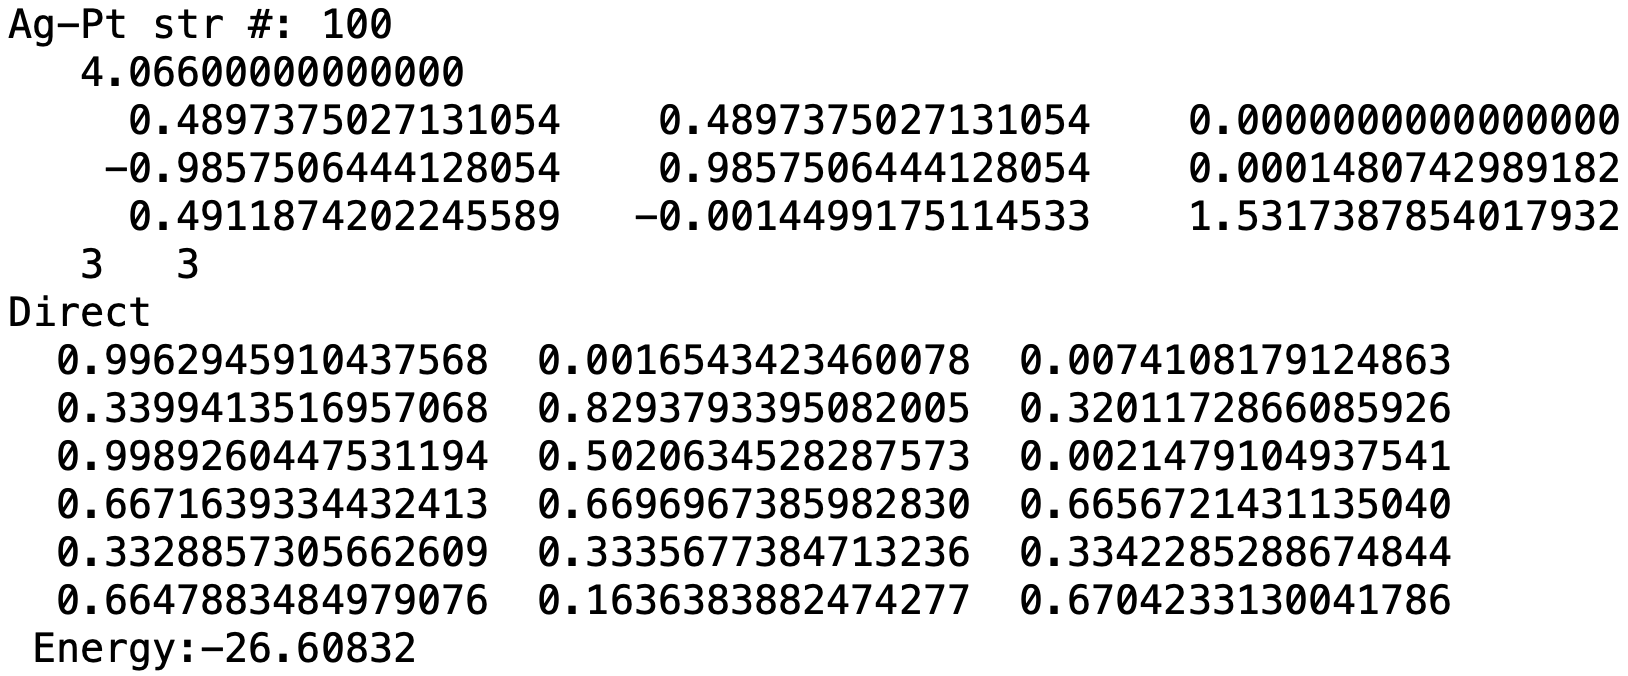
\includegraphics[scale = 0.3]{Figures/system2}
\caption{An example of the data given in AgPtdata.txt that needs to be used to build the model.
\label{system2data}} 
\end{figure}

\subsection{Model Construction}\label{Sect:procedureConstruction}
\par With the file parsed and the important data retrieved, the process of building a model can commence. The potential energy of a single particle is due to its interactions with all its surrounding particles, thus the unit cell must be propagated outwards in all three dimensions. All atomic pairs can be enumerated by adding multiples of the lattice vectors. Then the relative position of each affecting particle can be determined and the vector separating the particle pair can be calculated. These separation vectors are the information that will be passed into the basis function to construct the model. 
\par Because the affect two particles have on each other drop off as a function of distance, the unit cell does not need to be propogated infinitely in each direction, only out to a sphere of reasonable influence, beyond which all interactions are negligible. Clearly the choice of radius for said sphere will make a significant impact on the quality of the model. It is also obvious that the one arbitrarily chosen radius cannot be applied effectively to each unique system. A simple solution is to make the radius of this sphere of influence can be chosen to be the magnitude of the largest lattice vector multiplied by a constant. Later the effect of the constant on the model's precision can be tested, but for now will be chosen to be 1.2.
\par This simplification from the ``sphere of influence" gives a clear upper bound to our unit cell propagation. It is expected that the unit cell will be propagated out further than the radius in each direction, thus encapsulating said sphere. An example of this iterated unit cell can be seen in Figure \ref{iteratedUnitCells}. 

%\begin{figure}[h]
%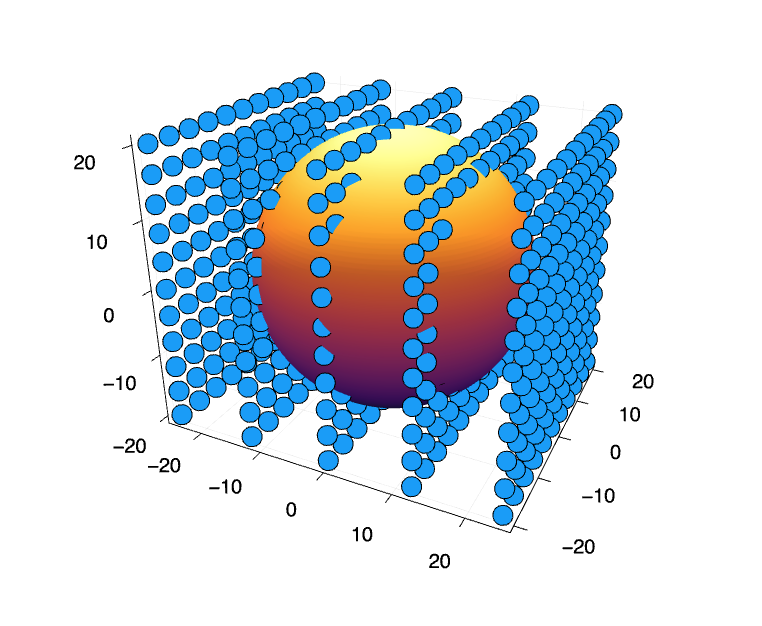
\includegraphics[scale = 0.65]{Figures/iteratedUnitCell}
%\caption{The sphere of influence for one silver atom is completely encapsulated by the unit cell's iterations. Only one particle from each unit cell is shown.
%\label{iteratedUnitCell}} 
%\end{figure}

\begin{figure}
  \begin{subfigure}{0.47\textwidth}
    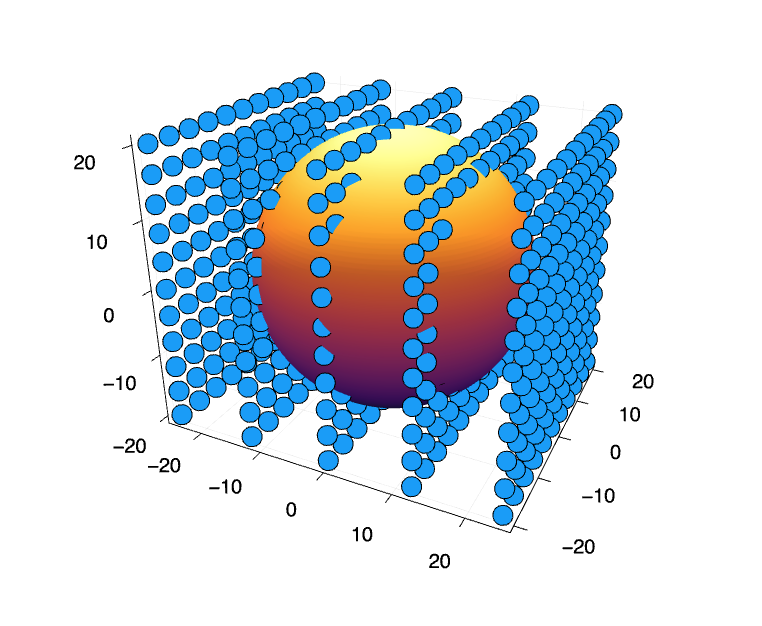
\includegraphics[width=\linewidth]{Figures/iteratedUnitCell}
    %\caption{First subfigure} 
    \label{iteratedUnitCellFirst}
  \end{subfigure}%
  \\
  %\hspace*{\fill}   % maximize separation between the subfigures
  \begin{subfigure}{0.45\textwidth}
    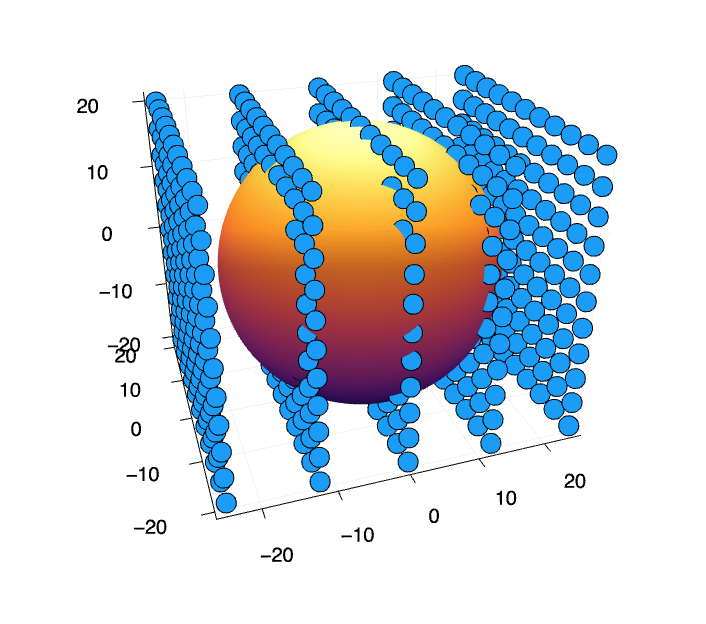
\includegraphics[width=\linewidth]{Figures/iteratedUnitCell2}
    %\caption{Second subfigure} 
    \label{iteratedUnitCellSecond}
  \end{subfigure}%

\caption{The sphere of influence for one silver atom is completely encapsulated by the unit cell's iterations from two different perspectives. Only one particle from each unit cell is shown.} \label{iteratedUnitCells}
\end{figure}


Now each of the unit cells in Figure \ref{iteratedUnitCells} can be populated with all the atoms contained within. From that fully populated unit cell can be extracted only the atoms inside the sphere. When these atoms are stored into a new vector, they can be re-plotted as in Figure \ref{plotAgAtomSphere}. When this process is repeated for every system in the given data, the result is a vector containing these ``important positions" for each unique silver and platinum atom in each unit cell. The separation vectors can be quickly calculated and their norms stored in three separate vectors, one for each type of interaction (Ag-Ag, Pt-Pt, and Ag-Pt). 

\begin{figure}[h]
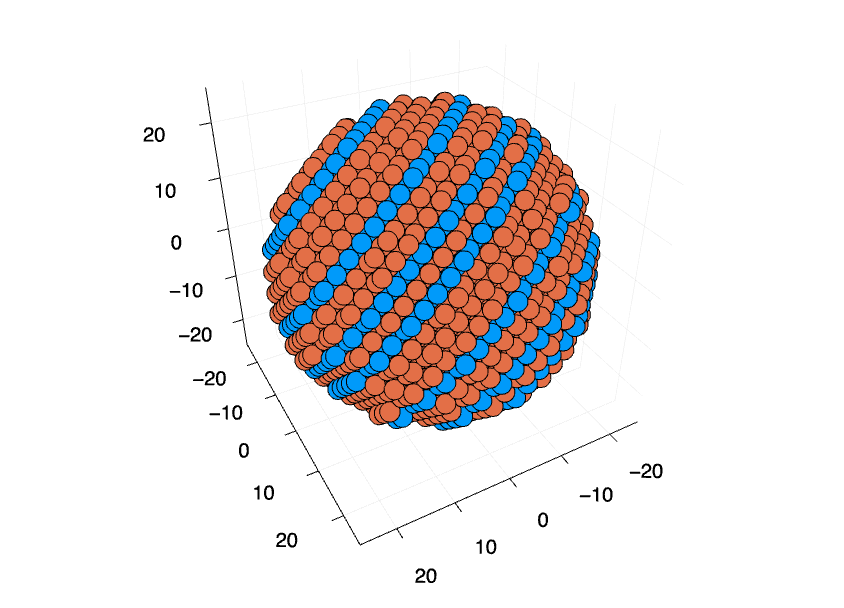
\includegraphics[scale = 0.6]{Figures/plotAgAtomSphere(3,1)}
\caption{Every silver and platinum atom inside the sphere of interest. According to the model, these are the only atoms interacting with the central atom in question. This data is taken from the first silver atom in the third sample system. 
\label{plotAgAtomSphere}} 
\end{figure}

With all the pertinent information from the data set organized into vectors, composition of the $A$ matrix can begin. As in the corollary Lennard-Jones example, each row represents a crystal structure and each column corresponds to a unique basis function. Also as in the Lennard-Jones code, a single basis function will result in three columns of $A$ due to each type of interaction. With 300 basis functions, the first 300 columns will be calculated using 300 unique basis functions with separation vector norms from Ag-Ag interactions. The following 300 columns from Pt-Pt interactions and the final 300 from Ag-Pt. The size of the training set is limited to 1224, the number of systems given in the data set. Whatever systems are not included in the training set will comprise the holdout set.
\par The basis functions will again be chosen to be bessel functions of the second kind. This is because of the similarity in potential energy between two atoms as a function of distance and the shape of the graph of said bessel functions. 
\par Once the model is fully constructed, tests can be run to determine the effect of radius, sample number, and number of basis functions on the precision and accuracy of the model. An increase of radius, sample number, or number of basis functions will make significant impacts on the program runtime. As the radius is increased, the unit cell must be propagated out further and more atom interactions considered. Thus effect of the radius will drastically impact the total runtime. For every basis function added, there will be three columns added to the $A$ matrix, drawing out its composition and calculation times. 
\par Generally, as the number of basis functions is increased and the radius of influence extended, the model's predictions will become increasingly reliable. On the other hand, as those factors increase accuracy and precision, they also increase the computational costs. It would be ideal to find a manageable trade off between the program's runtime and reliability. To investigate the quality of the model as a function of cutoff radius, sample number, and number of basis functions, a sweep can be conducted over a range of values for each and record the details of the fit for each combination. Rather than run this code for weeks on a normal desktop computer, it was completed on Mary Lou, BYU's supercomputer. 


%\begin{figure}
%  \begin{subfigure}{0.45\textwidth}
%    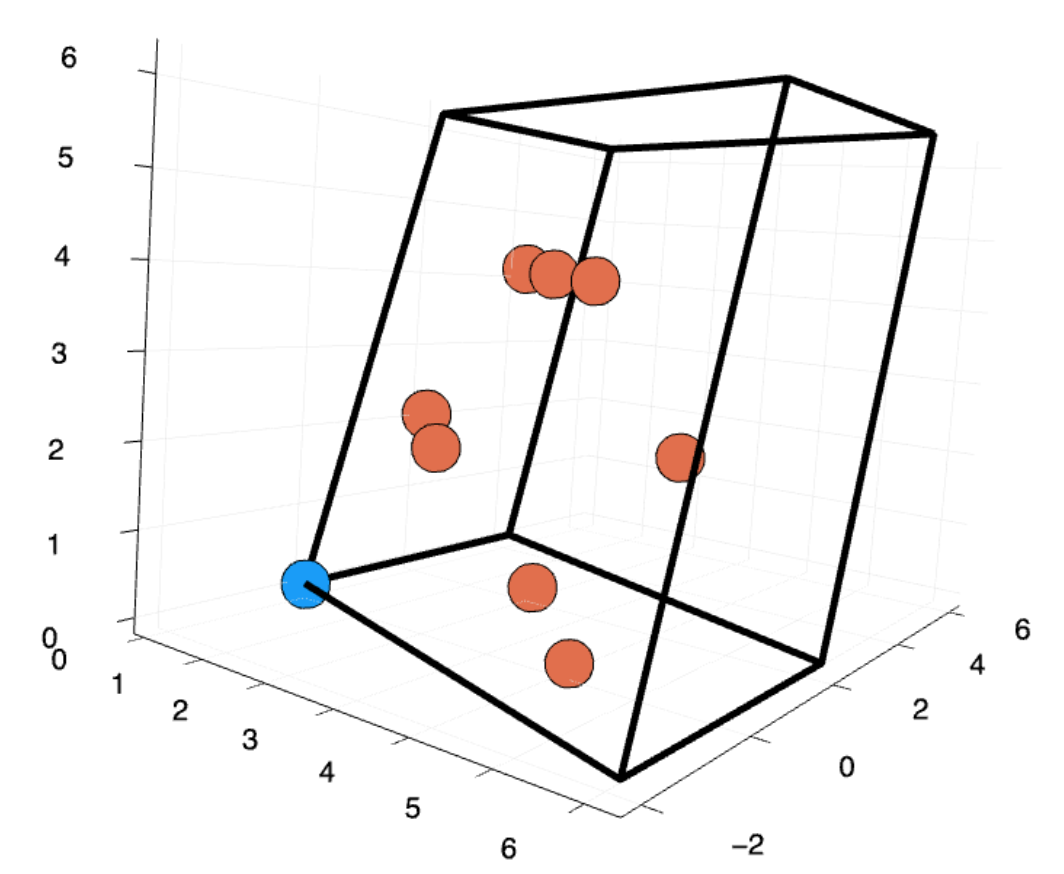
\includegraphics[width=\linewidth]{Figures/primitiveCell1}
%    %\caption{First subfigure} 
%    \label{primitiveFirst}
%  \end{subfigure}%
%  \\
%  %\hspace*{\fill}   % maximize separation between the subfigures
%  \begin{subfigure}{0.45\textwidth}
%    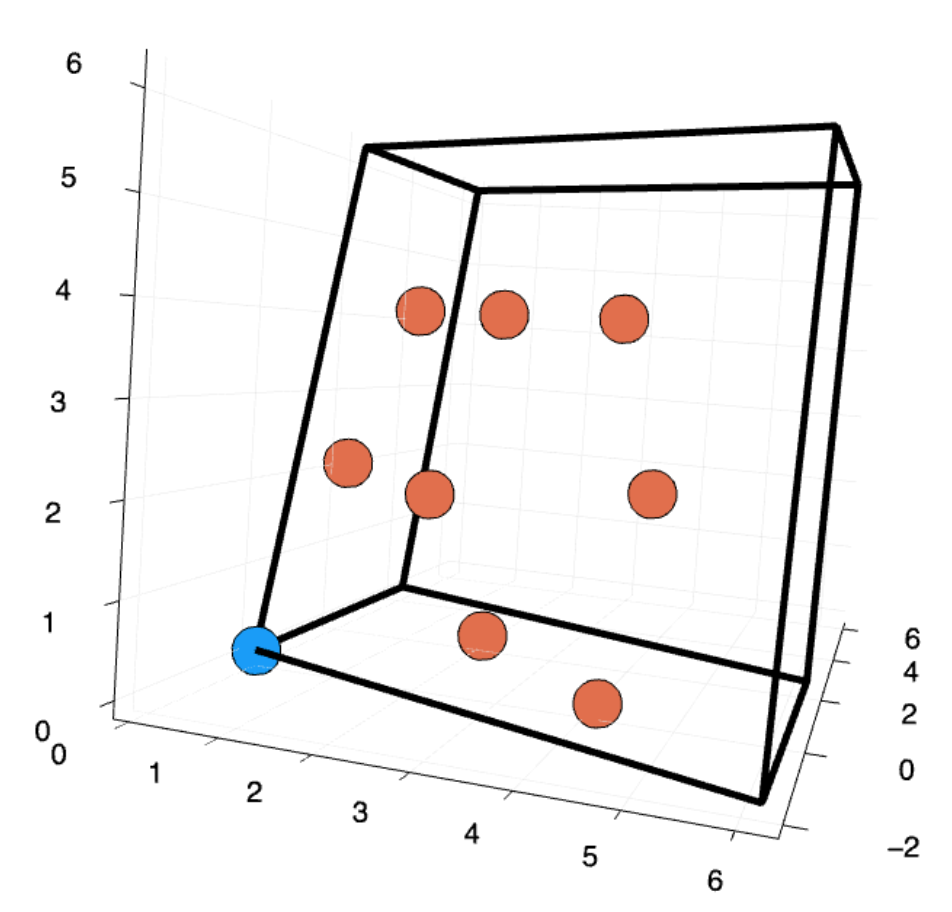
\includegraphics[width=\linewidth]{Figures/primitiveCell2}
%    %\caption{Second subfigure} 
%    \label{primitiveSecond}
%  \end{subfigure}%
%  \\
%  %\hspace*{\fill}   % maximize separation between the subfigures
%  \begin{subfigure}{0.45\textwidth}
%    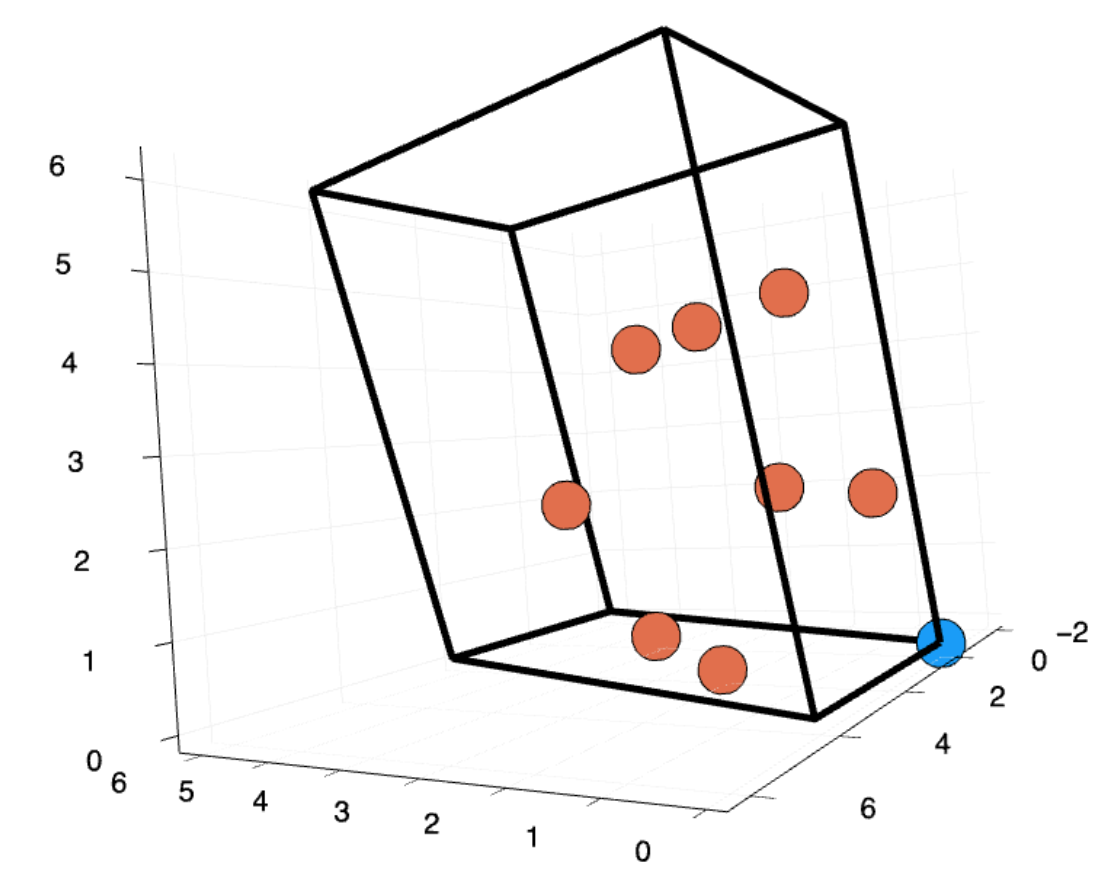
\includegraphics[width=\linewidth]{Figures/primitiveCell3}
%    %\caption{Second subfigure} 
%    \label{primitiveThird}
%  \end{subfigure}
%
%\caption{The primitive unit cell for configuration 65 from three different perspectives. The blue point is the single Ag atom while each red point shows each Pt atom in said configuration.} \label{primitiveUnitCells}
%\end{figure}
